\documentclass[twoside]{book}

% Packages required by doxygen
\usepackage{fixltx2e}
\usepackage{calc}
\usepackage{doxygen}
\usepackage[export]{adjustbox} % also loads graphicx
\usepackage{graphicx}
\usepackage[utf8]{inputenc}
\usepackage{makeidx}
\usepackage{multicol}
\usepackage{multirow}
\PassOptionsToPackage{warn}{textcomp}
\usepackage{textcomp}
\usepackage[nointegrals]{wasysym}
\usepackage[table]{xcolor}

% Font selection
\usepackage[T1]{fontenc}
\usepackage[scaled=.90]{helvet}
\usepackage{courier}
\usepackage{amssymb}
\usepackage{sectsty}
\renewcommand{\familydefault}{\sfdefault}
\allsectionsfont{%
  \fontseries{bc}\selectfont%
  \color{darkgray}%
}
\renewcommand{\DoxyLabelFont}{%
  \fontseries{bc}\selectfont%
  \color{darkgray}%
}
\newcommand{\+}{\discretionary{\mbox{\scriptsize$\hookleftarrow$}}{}{}}

% Page & text layout
\usepackage{geometry}
\geometry{%
  a4paper,%
  top=2.5cm,%
  bottom=2.5cm,%
  left=2.5cm,%
  right=2.5cm%
}
\tolerance=750
\hfuzz=15pt
\hbadness=750
\setlength{\emergencystretch}{15pt}
\setlength{\parindent}{0cm}
\setlength{\parskip}{0.2cm}
\makeatletter
\renewcommand{\paragraph}{%
  \@startsection{paragraph}{4}{0ex}{-1.0ex}{1.0ex}{%
    \normalfont\normalsize\bfseries\SS@parafont%
  }%
}
\renewcommand{\subparagraph}{%
  \@startsection{subparagraph}{5}{0ex}{-1.0ex}{1.0ex}{%
    \normalfont\normalsize\bfseries\SS@subparafont%
  }%
}
\makeatother

% Headers & footers
\usepackage{fancyhdr}
\pagestyle{fancyplain}
\fancyhead[LE]{\fancyplain{}{\bfseries\thepage}}
\fancyhead[CE]{\fancyplain{}{}}
\fancyhead[RE]{\fancyplain{}{\bfseries\leftmark}}
\fancyhead[LO]{\fancyplain{}{\bfseries\rightmark}}
\fancyhead[CO]{\fancyplain{}{}}
\fancyhead[RO]{\fancyplain{}{\bfseries\thepage}}
\fancyfoot[LE]{\fancyplain{}{}}
\fancyfoot[CE]{\fancyplain{}{}}
\fancyfoot[RE]{\fancyplain{}{\bfseries\scriptsize Generated on Wed May 11 2016 19\+:49\+:40 for My Project by Doxygen }}
\fancyfoot[LO]{\fancyplain{}{\bfseries\scriptsize Generated on Wed May 11 2016 19\+:49\+:40 for My Project by Doxygen }}
\fancyfoot[CO]{\fancyplain{}{}}
\fancyfoot[RO]{\fancyplain{}{}}
\renewcommand{\footrulewidth}{0.4pt}
\renewcommand{\chaptermark}[1]{%
  \markboth{#1}{}%
}
\renewcommand{\sectionmark}[1]{%
  \markright{\thesection\ #1}%
}

% Indices & bibliography
\usepackage{natbib}
\usepackage[titles]{tocloft}
\setcounter{tocdepth}{3}
\setcounter{secnumdepth}{5}
\makeindex

% Hyperlinks (required, but should be loaded last)
\usepackage{ifpdf}
\ifpdf
  \usepackage[pdftex,pagebackref=true]{hyperref}
\else
  \usepackage[ps2pdf,pagebackref=true]{hyperref}
\fi
\hypersetup{%
  colorlinks=true,%
  linkcolor=blue,%
  citecolor=blue,%
  unicode%
}

% Custom commands
\newcommand{\clearemptydoublepage}{%
  \newpage{\pagestyle{empty}\cleardoublepage}%
}


%===== C O N T E N T S =====

\begin{document}

% Titlepage & ToC
\hypersetup{pageanchor=false,
             bookmarks=true,
             bookmarksnumbered=true,
             pdfencoding=unicode
            }
\pagenumbering{roman}
\begin{titlepage}
\vspace*{7cm}
\begin{center}%
{\Large My Project }\\
\vspace*{1cm}
{\large Generated by Doxygen 1.8.9.1}\\
\vspace*{0.5cm}
{\small Wed May 11 2016 19:49:40}\\
\end{center}
\end{titlepage}
\clearemptydoublepage
\tableofcontents
\clearemptydoublepage
\pagenumbering{arabic}
\hypersetup{pageanchor=true}

%--- Begin generated contents ---
\chapter{File Index}
\section{File List}
Here is a list of all documented files with brief descriptions\+:\begin{DoxyCompactList}
\item\contentsline{section}{\hyperlink{main_8c}{main.\+c} }{\pageref{main_8c}}{}
\end{DoxyCompactList}

\chapter{File Documentation}
\hypertarget{main_8c}{}\section{main.\+c File Reference}
\label{main_8c}\index{main.\+c@{main.\+c}}
{\ttfamily \#include \char`\"{}S\+D\+L/\+S\+D\+L.\+h\char`\"{}}\\*
{\ttfamily \#include \char`\"{}S\+D\+L/\+S\+D\+L\+\_\+image.\+h\char`\"{}}\\*
{\ttfamily \#include \char`\"{}stdio.\+h\char`\"{}}\\*
{\ttfamily \#include $<$string.\+h$>$}\\*
{\ttfamily \#include $<$S\+D\+L/\+S\+D\+L\+\_\+ttf.\+h$>$}\\*
{\ttfamily \#include $<$time.\+h$>$}\\*
{\ttfamily \#include $<$S\+D\+L/\+S\+D\+L\+\_\+mixer.\+h$>$}\\*
Include dependency graph for main.\+c\+:\nopagebreak
\begin{figure}[H]
\begin{center}
\leavevmode
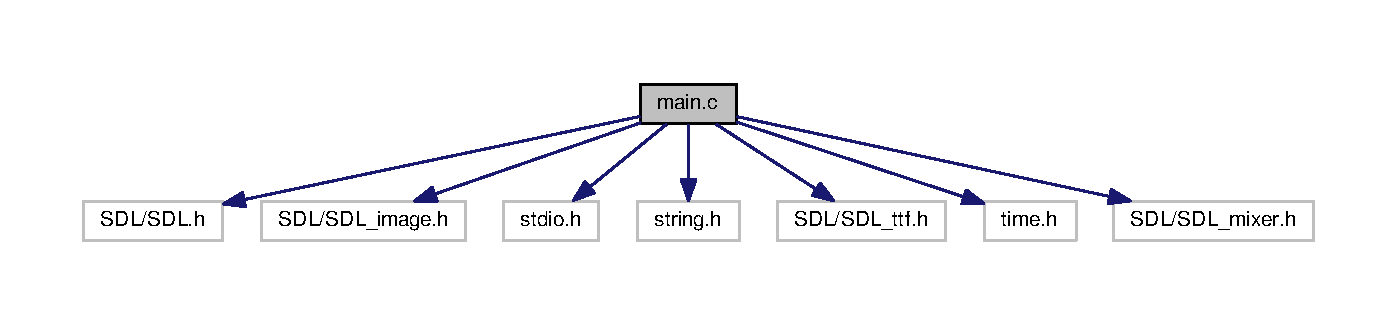
\includegraphics[width=350pt]{main_8c__incl}
\end{center}
\end{figure}
\subsection*{Functions}
\begin{DoxyCompactItemize}
\item 
void \hyperlink{main_8c_a4f6226920d40f28f7eb399376733058e}{option} ()
\item 
int \hyperlink{main_8c_a4c211d62aeddbe950f99c86fd347f71e}{Pmenu} (int $\ast$action)
\begin{DoxyCompactList}\small\item\em Le menu principal qui s\textquotesingle{}affiche au lancement du jeu. \end{DoxyCompactList}\item 
void \hyperlink{main_8c_ad7207e18573041d0a7fa144594016abe}{Smain} (int $\ast$cond)
\begin{DoxyCompactList}\small\item\em Le sous menu qui s\textquotesingle{}afficher en cliquant sur echap dans le jeu. \end{DoxyCompactList}\item 
void \hyperlink{main_8c_a8ab296dd84181c3393e2082777ccc350}{apply\+\_\+surface} (int x, int y, S\+D\+L\+\_\+\+Surface $\ast$source, S\+D\+L\+\_\+\+Surface $\ast$destination)
\item 
int \hyperlink{main_8c_a05848de25ac2dbec233935058a1d24b4}{init} ()
\begin{DoxyCompactList}\small\item\em Initialisation (video , texte , ..) \end{DoxyCompactList}\item 
S\+D\+L\+\_\+\+Surface $\ast$ \hyperlink{main_8c_adc9f1cd6c730a0d793d64ccee1270747}{load\+\_\+image} (char $\ast$nom)
\begin{DoxyCompactList}\small\item\em Optimization d\textquotesingle{}une image. \end{DoxyCompactList}\item 
int \hyperlink{main_8c_a8a47b8642736fcad746fbac37ca33d5c}{load\+\_\+files} ()
\begin{DoxyCompactList}\small\item\em Charger les images (La map , le background concernant la collision) \end{DoxyCompactList}\item 
void \hyperlink{main_8c_ada7f892aa09adca3647631590ca1beb0}{clean\+\_\+up} ()
\item 
S\+D\+L\+\_\+\+Rect \hyperlink{main_8c_ae729f900628d2f95f9feaf4943c8190f}{limit} (int x, int y)
\item 
S\+D\+L\+\_\+\+Surface $\ast$ \hyperlink{main_8c_ac1c080d2479fb838b42bd3d95ce40d90}{anim\+\_\+right} (int $\ast$mouvement)
\begin{DoxyCompactList}\small\item\em Animation du personnage. \end{DoxyCompactList}\item 
S\+D\+L\+\_\+\+Surface $\ast$ \hyperlink{main_8c_a13b737c365398803efde61c82d2eff21}{anim\+\_\+left} (int $\ast$mouvement)
\begin{DoxyCompactList}\small\item\em Animation du personnage. \end{DoxyCompactList}\item 
S\+D\+L\+\_\+\+Surface $\ast$ \hyperlink{main_8c_ac0c665600daeff33bec62abf58fb5c33}{anim\+\_\+up} (int $\ast$mouvement)
\begin{DoxyCompactList}\small\item\em Animation du personnage. \end{DoxyCompactList}\item 
S\+D\+L\+\_\+\+Surface $\ast$ \hyperlink{main_8c_aa21866949710887de7c0dd5bb1a30378}{anim\+\_\+down} (int $\ast$mouvement)
\begin{DoxyCompactList}\small\item\em Animation du personnage. \end{DoxyCompactList}\item 
S\+D\+L\+\_\+\+Color \hyperlink{main_8c_a9ec79b71532402381966fc93325d3e52}{Get\+Pixel} (S\+D\+L\+\_\+\+Surface $\ast$p\+Surface, int x, int y)
\item 
int \hyperlink{main_8c_aa71223ae8f9dfe12e7b6f04648a7cb5a}{detecter\+\_\+collision\+\_\+background} (S\+D\+L\+\_\+\+Surface $\ast$image, S\+D\+L\+\_\+\+Rect position)
\begin{DoxyCompactList}\small\item\em detecteur de collision \end{DoxyCompactList}\item 
int \hyperlink{main_8c_a50171e8ac1cb26d2f74ff8c9622554c0}{detecter\+\_\+\+Pin} (S\+D\+L\+\_\+\+Surface $\ast$image, S\+D\+L\+\_\+\+Rect position)
\item 
int \hyperlink{main_8c_aeeb063d6f84375e9104a18121167c05c}{detecter\+\_\+collision\+\_\+restaurant} (S\+D\+L\+\_\+\+Surface $\ast$image, S\+D\+L\+\_\+\+Rect position)
\begin{DoxyCompactList}\small\item\em detecter si le personnage est placé devant le restaurant (dans le jeu) \end{DoxyCompactList}\item 
void \hyperlink{main_8c_afc674cf16befffaaa68ae85afda7ec97}{sauvegarde} (S\+D\+L\+\_\+\+Rect $\ast$bg)
\begin{DoxyCompactList}\small\item\em Sauvegarde. \end{DoxyCompactList}\item 
void \hyperlink{main_8c_a3b1181818908fea5d147d63129f3f553}{Score} (int vie, int t\+\_\+ennemis\mbox{[}$\,$\mbox{]}, S\+D\+L\+\_\+\+Rect $\ast$pospers)
\item 
void \hyperlink{main_8c_aae0562b412c426274e3d1533b59c92c2}{Reunion} ()
\begin{DoxyCompactList}\small\item\em Assure l\textquotesingle{}entrée du personnage dans le restaurant (jeu) et affiche l\textquotesingle{}ensemble de question que lui seront posées. \end{DoxyCompactList}\item 
void \hyperlink{main_8c_a320de47948ac1ffb0b721f637f28fc4a}{afficherscore} (int score)
\item 
void \hyperlink{main_8c_a1c133b804ee89ec0b7a9ba892501ceaa}{pershud} (int score)
\begin{DoxyCompactList}\small\item\em Afficher le score au dessus du personnage dans le jeu. \end{DoxyCompactList}\item 
void \hyperlink{main_8c_a540b69bbd3c9f6c0b15aaef898d0535e}{afficherpin} (S\+D\+L\+\_\+\+Surface $\ast$destination)
\item 
void \hyperlink{main_8c_aa0e9e94095fa1121dec0aae2d9512759}{afficher\+\_\+ennemi} (S\+D\+L\+\_\+\+Surface $\ast$car1, S\+D\+L\+\_\+\+Surface $\ast$car2, S\+D\+L\+\_\+\+Surface $\ast$\hyperlink{main_8c_a96eebd19c7cea6af7e50e821d04ed494}{fenetre}, S\+D\+L\+\_\+\+Rect t\+\_\+ennemis\mbox{[}$\,$\mbox{]})
\begin{DoxyCompactList}\small\item\em affichage des ennemies \end{DoxyCompactList}\item 
int \hyperlink{main_8c_a008b92b9fa8fe060603dc3339b1866b4}{arduino\+Read\+Data} (char $\ast$c)
\begin{DoxyCompactList}\small\item\em Lire les données depuis Arduino. \end{DoxyCompactList}\item 
int \hyperlink{main_8c_a62cf5a4f7c5a9956f0acfdcf39d28aff}{arduino\+Write\+Data} (int k)
\begin{DoxyCompactList}\small\item\em Envoyer des données vers Arduino. \end{DoxyCompactList}\item 
void \hyperlink{main_8c_acb123aa507c7819b41273af064d04987}{mvt\+\_\+arduino} (S\+D\+L\+\_\+\+Rect $\ast$bg, S\+D\+L\+\_\+\+Surface $\ast$\hyperlink{main_8c_a99ec2450c32b6c9cd1cbd6d7d006f360}{image\+De\+Fond\+Collision}, S\+D\+L\+\_\+\+Rect $\ast$positionpers, int $\ast$mouvement, S\+D\+L\+\_\+\+Rect $\ast$pospers, S\+D\+L\+\_\+\+Surface $\ast$$\ast$image)
\begin{DoxyCompactList}\small\item\em Deplacement avec la manette (Arduino) \end{DoxyCompactList}\item 
void \hyperlink{main_8c_af13976bbb5c9020deac38ad2cc675658}{mvt\+\_\+clavier} (int $\ast$reun, S\+D\+L\+\_\+\+Surface $\ast$\hyperlink{main_8c_a96eebd19c7cea6af7e50e821d04ed494}{fenetre}, S\+D\+L\+Key bouton, S\+D\+L\+\_\+\+Rect $\ast$bg, S\+D\+L\+\_\+\+Surface $\ast$\hyperlink{main_8c_a99ec2450c32b6c9cd1cbd6d7d006f360}{image\+De\+Fond\+Collision}, S\+D\+L\+\_\+\+Rect $\ast$positionpers, int $\ast$mouvement, S\+D\+L\+\_\+\+Rect $\ast$pospers, S\+D\+L\+\_\+\+Surface $\ast$$\ast$image, int $\ast$ok, int $\ast$save)
\begin{DoxyCompactList}\small\item\em L\textquotesingle{}ensemble d\textquotesingle{}actions assurés par le clavier. \end{DoxyCompactList}\item 
int \hyperlink{main_8c_a700a0caa5b70a06d1064e576f9f3cf65}{main} (int argc, char $\ast$args\mbox{[}$\,$\mbox{]})
\begin{DoxyCompactList}\small\item\em Game\+Loop. \end{DoxyCompactList}\end{DoxyCompactItemize}
\subsection*{Variables}
\begin{DoxyCompactItemize}
\item 
const int \hyperlink{main_8c_afa589067d575acf741f604f4315408c6}{fenetre\+\_\+\+W\+I\+D\+T\+H} = 1300
\item 
const int \hyperlink{main_8c_ae3b9b4e33bfbda0d6cb71a5fec6d48ef}{fenetre\+\_\+\+H\+E\+I\+G\+H\+T} = 700
\item 
const int \hyperlink{main_8c_a1b094738dfdb96d32c70e63a72ba67fd}{fenetre\+\_\+\+B\+P\+P} = 32
\item 
const int \hyperlink{main_8c_abe06f96c5aeacdb02e4b66e34e609982}{F\+R\+A\+M\+E\+S\+\_\+\+P\+E\+R\+\_\+\+S\+E\+C\+O\+N\+D} = 50
\item 
S\+D\+L\+\_\+\+Surface $\ast$ \hyperlink{main_8c_a68389876c2746622931d187c587f9c4d}{background} = N\+U\+L\+L
\item 
S\+D\+L\+\_\+\+Surface $\ast$ \hyperlink{main_8c_a99ec2450c32b6c9cd1cbd6d7d006f360}{image\+De\+Fond\+Collision} =N\+U\+L\+L
\item 
S\+D\+L\+\_\+\+Surface $\ast$ \hyperlink{main_8c_a96eebd19c7cea6af7e50e821d04ed494}{fenetre} = N\+U\+L\+L
\item 
S\+D\+L\+\_\+\+Event \hyperlink{main_8c_a6b57f01d3c576db5368dd0efc2f435a4}{event}
\end{DoxyCompactItemize}


\subsection{Function Documentation}
\hypertarget{main_8c_aa0e9e94095fa1121dec0aae2d9512759}{}\index{main.\+c@{main.\+c}!afficher\+\_\+ennemi@{afficher\+\_\+ennemi}}
\index{afficher\+\_\+ennemi@{afficher\+\_\+ennemi}!main.\+c@{main.\+c}}
\subsubsection[{afficher\+\_\+ennemi}]{\setlength{\rightskip}{0pt plus 5cm}void afficher\+\_\+ennemi (
\begin{DoxyParamCaption}
\item[{S\+D\+L\+\_\+\+Surface $\ast$}]{car1, }
\item[{S\+D\+L\+\_\+\+Surface $\ast$}]{car2, }
\item[{S\+D\+L\+\_\+\+Surface $\ast$}]{fenetre, }
\item[{S\+D\+L\+\_\+\+Rect}]{t\+\_\+ennemis\mbox{[}$\,$\mbox{]}}
\end{DoxyParamCaption}
)}\label{main_8c_aa0e9e94095fa1121dec0aae2d9512759}


affichage des ennemies 

\hypertarget{main_8c_a540b69bbd3c9f6c0b15aaef898d0535e}{}\index{main.\+c@{main.\+c}!afficherpin@{afficherpin}}
\index{afficherpin@{afficherpin}!main.\+c@{main.\+c}}
\subsubsection[{afficherpin}]{\setlength{\rightskip}{0pt plus 5cm}void afficherpin (
\begin{DoxyParamCaption}
\item[{S\+D\+L\+\_\+\+Surface $\ast$}]{destination}
\end{DoxyParamCaption}
)}\label{main_8c_a540b69bbd3c9f6c0b15aaef898d0535e}
\hypertarget{main_8c_a320de47948ac1ffb0b721f637f28fc4a}{}\index{main.\+c@{main.\+c}!afficherscore@{afficherscore}}
\index{afficherscore@{afficherscore}!main.\+c@{main.\+c}}
\subsubsection[{afficherscore}]{\setlength{\rightskip}{0pt plus 5cm}void afficherscore (
\begin{DoxyParamCaption}
\item[{int}]{score}
\end{DoxyParamCaption}
)}\label{main_8c_a320de47948ac1ffb0b721f637f28fc4a}
\hypertarget{main_8c_aa21866949710887de7c0dd5bb1a30378}{}\index{main.\+c@{main.\+c}!anim\+\_\+down@{anim\+\_\+down}}
\index{anim\+\_\+down@{anim\+\_\+down}!main.\+c@{main.\+c}}
\subsubsection[{anim\+\_\+down}]{\setlength{\rightskip}{0pt plus 5cm}S\+D\+L\+\_\+\+Surface$\ast$ anim\+\_\+down (
\begin{DoxyParamCaption}
\item[{int $\ast$}]{mouvement}
\end{DoxyParamCaption}
)}\label{main_8c_aa21866949710887de7c0dd5bb1a30378}


Animation du personnage. 


\begin{DoxyParams}{Parameters}
{\em $\ast$mouvement} & \+: gauche , droite , haut , bas\\
\hline
\end{DoxyParams}
\begin{DoxyReturn}{Returns}
animation 
\end{DoxyReturn}


Here is the caller graph for this function\+:
\nopagebreak
\begin{figure}[H]
\begin{center}
\leavevmode
\includegraphics[width=326pt]{main_8c_aa21866949710887de7c0dd5bb1a30378_icgraph}
\end{center}
\end{figure}


\hypertarget{main_8c_a13b737c365398803efde61c82d2eff21}{}\index{main.\+c@{main.\+c}!anim\+\_\+left@{anim\+\_\+left}}
\index{anim\+\_\+left@{anim\+\_\+left}!main.\+c@{main.\+c}}
\subsubsection[{anim\+\_\+left}]{\setlength{\rightskip}{0pt plus 5cm}S\+D\+L\+\_\+\+Surface$\ast$ anim\+\_\+left (
\begin{DoxyParamCaption}
\item[{int $\ast$}]{mouvement}
\end{DoxyParamCaption}
)}\label{main_8c_a13b737c365398803efde61c82d2eff21}


Animation du personnage. 


\begin{DoxyParams}{Parameters}
{\em $\ast$mouvement} & \+: gauche , droite , haut , bas\\
\hline
\end{DoxyParams}
\begin{DoxyReturn}{Returns}
animation 
\end{DoxyReturn}


Here is the caller graph for this function\+:
\nopagebreak
\begin{figure}[H]
\begin{center}
\leavevmode
\includegraphics[width=316pt]{main_8c_a13b737c365398803efde61c82d2eff21_icgraph}
\end{center}
\end{figure}


\hypertarget{main_8c_ac1c080d2479fb838b42bd3d95ce40d90}{}\index{main.\+c@{main.\+c}!anim\+\_\+right@{anim\+\_\+right}}
\index{anim\+\_\+right@{anim\+\_\+right}!main.\+c@{main.\+c}}
\subsubsection[{anim\+\_\+right}]{\setlength{\rightskip}{0pt plus 5cm}S\+D\+L\+\_\+\+Surface$\ast$ anim\+\_\+right (
\begin{DoxyParamCaption}
\item[{int $\ast$}]{mouvement}
\end{DoxyParamCaption}
)}\label{main_8c_ac1c080d2479fb838b42bd3d95ce40d90}


Animation du personnage. 


\begin{DoxyParams}{Parameters}
{\em $\ast$mouvement} & \+: gauche , droite , haut , bas\\
\hline
\end{DoxyParams}
\begin{DoxyReturn}{Returns}
animation 
\end{DoxyReturn}


Here is the caller graph for this function\+:
\nopagebreak
\begin{figure}[H]
\begin{center}
\leavevmode
\includegraphics[width=322pt]{main_8c_ac1c080d2479fb838b42bd3d95ce40d90_icgraph}
\end{center}
\end{figure}


\hypertarget{main_8c_ac0c665600daeff33bec62abf58fb5c33}{}\index{main.\+c@{main.\+c}!anim\+\_\+up@{anim\+\_\+up}}
\index{anim\+\_\+up@{anim\+\_\+up}!main.\+c@{main.\+c}}
\subsubsection[{anim\+\_\+up}]{\setlength{\rightskip}{0pt plus 5cm}S\+D\+L\+\_\+\+Surface$\ast$ anim\+\_\+up (
\begin{DoxyParamCaption}
\item[{int $\ast$}]{mouvement}
\end{DoxyParamCaption}
)}\label{main_8c_ac0c665600daeff33bec62abf58fb5c33}


Animation du personnage. 


\begin{DoxyParams}{Parameters}
{\em $\ast$mouvement} & \+: gauche , droite , haut , bas\\
\hline
\end{DoxyParams}
\begin{DoxyReturn}{Returns}
animation 
\end{DoxyReturn}


Here is the caller graph for this function\+:
\nopagebreak
\begin{figure}[H]
\begin{center}
\leavevmode
\includegraphics[width=313pt]{main_8c_ac0c665600daeff33bec62abf58fb5c33_icgraph}
\end{center}
\end{figure}


\hypertarget{main_8c_a8ab296dd84181c3393e2082777ccc350}{}\index{main.\+c@{main.\+c}!apply\+\_\+surface@{apply\+\_\+surface}}
\index{apply\+\_\+surface@{apply\+\_\+surface}!main.\+c@{main.\+c}}
\subsubsection[{apply\+\_\+surface}]{\setlength{\rightskip}{0pt plus 5cm}void apply\+\_\+surface (
\begin{DoxyParamCaption}
\item[{int}]{x, }
\item[{int}]{y, }
\item[{S\+D\+L\+\_\+\+Surface $\ast$}]{source, }
\item[{S\+D\+L\+\_\+\+Surface $\ast$}]{destination}
\end{DoxyParamCaption}
)}\label{main_8c_a8ab296dd84181c3393e2082777ccc350}

\begin{DoxyParams}{Parameters}
{\em x} & \\
\hline
{\em y} & \\
\hline
\end{DoxyParams}
\begin{DoxyReturn}{Returns}
Void 
\end{DoxyReturn}


Here is the caller graph for this function\+:
\nopagebreak
\begin{figure}[H]
\begin{center}
\leavevmode
\includegraphics[width=231pt]{main_8c_a8ab296dd84181c3393e2082777ccc350_icgraph}
\end{center}
\end{figure}


\hypertarget{main_8c_a008b92b9fa8fe060603dc3339b1866b4}{}\index{main.\+c@{main.\+c}!arduino\+Read\+Data@{arduino\+Read\+Data}}
\index{arduino\+Read\+Data@{arduino\+Read\+Data}!main.\+c@{main.\+c}}
\subsubsection[{arduino\+Read\+Data}]{\setlength{\rightskip}{0pt plus 5cm}int arduino\+Read\+Data (
\begin{DoxyParamCaption}
\item[{char $\ast$}]{c}
\end{DoxyParamCaption}
)}\label{main_8c_a008b92b9fa8fe060603dc3339b1866b4}


Lire les données depuis Arduino. 


\begin{DoxyParams}{Parameters}
{\em $\ast$c} & \+: donnée\\
\hline
\end{DoxyParams}
\begin{DoxyReturn}{Returns}
0 \+: si oui 

-\/1 \+: si non 
\end{DoxyReturn}


Here is the caller graph for this function\+:
\nopagebreak
\begin{figure}[H]
\begin{center}
\leavevmode
\includegraphics[width=350pt]{main_8c_a008b92b9fa8fe060603dc3339b1866b4_icgraph}
\end{center}
\end{figure}


\hypertarget{main_8c_a62cf5a4f7c5a9956f0acfdcf39d28aff}{}\index{main.\+c@{main.\+c}!arduino\+Write\+Data@{arduino\+Write\+Data}}
\index{arduino\+Write\+Data@{arduino\+Write\+Data}!main.\+c@{main.\+c}}
\subsubsection[{arduino\+Write\+Data}]{\setlength{\rightskip}{0pt plus 5cm}int arduino\+Write\+Data (
\begin{DoxyParamCaption}
\item[{int}]{k}
\end{DoxyParamCaption}
)}\label{main_8c_a62cf5a4f7c5a9956f0acfdcf39d28aff}


Envoyer des données vers Arduino. 


\begin{DoxyParams}{Parameters}
{\em $\ast$c} & \+: donnée\\
\hline
\end{DoxyParams}
\begin{DoxyReturn}{Returns}
0 \+: si oui 

-\/1 \+: si non 
\end{DoxyReturn}
\hypertarget{main_8c_ada7f892aa09adca3647631590ca1beb0}{}\index{main.\+c@{main.\+c}!clean\+\_\+up@{clean\+\_\+up}}
\index{clean\+\_\+up@{clean\+\_\+up}!main.\+c@{main.\+c}}
\subsubsection[{clean\+\_\+up}]{\setlength{\rightskip}{0pt plus 5cm}void clean\+\_\+up (
\begin{DoxyParamCaption}
{}
\end{DoxyParamCaption}
)}\label{main_8c_ada7f892aa09adca3647631590ca1beb0}


Here is the caller graph for this function\+:
\nopagebreak
\begin{figure}[H]
\begin{center}
\leavevmode
\includegraphics[width=210pt]{main_8c_ada7f892aa09adca3647631590ca1beb0_icgraph}
\end{center}
\end{figure}


\hypertarget{main_8c_aa71223ae8f9dfe12e7b6f04648a7cb5a}{}\index{main.\+c@{main.\+c}!detecter\+\_\+collision\+\_\+background@{detecter\+\_\+collision\+\_\+background}}
\index{detecter\+\_\+collision\+\_\+background@{detecter\+\_\+collision\+\_\+background}!main.\+c@{main.\+c}}
\subsubsection[{detecter\+\_\+collision\+\_\+background}]{\setlength{\rightskip}{0pt plus 5cm}int detecter\+\_\+collision\+\_\+background (
\begin{DoxyParamCaption}
\item[{S\+D\+L\+\_\+\+Surface $\ast$}]{image, }
\item[{S\+D\+L\+\_\+\+Rect}]{position}
\end{DoxyParamCaption}
)}\label{main_8c_aa71223ae8f9dfe12e7b6f04648a7cb5a}


detecteur de collision 


\begin{DoxyParams}{Parameters}
{\em $\ast$image} & \+: image du background de la collision \\
\hline
{\em position} & \+: position du personnage\\
\hline
\end{DoxyParams}
\begin{DoxyReturn}{Returns}
animation 
\end{DoxyReturn}


Here is the call graph for this function\+:
\nopagebreak
\begin{figure}[H]
\begin{center}
\leavevmode
\includegraphics[width=262pt]{main_8c_aa71223ae8f9dfe12e7b6f04648a7cb5a_cgraph}
\end{center}
\end{figure}




Here is the caller graph for this function\+:
\nopagebreak
\begin{figure}[H]
\begin{center}
\leavevmode
\includegraphics[width=350pt]{main_8c_aa71223ae8f9dfe12e7b6f04648a7cb5a_icgraph}
\end{center}
\end{figure}


\hypertarget{main_8c_aeeb063d6f84375e9104a18121167c05c}{}\index{main.\+c@{main.\+c}!detecter\+\_\+collision\+\_\+restaurant@{detecter\+\_\+collision\+\_\+restaurant}}
\index{detecter\+\_\+collision\+\_\+restaurant@{detecter\+\_\+collision\+\_\+restaurant}!main.\+c@{main.\+c}}
\subsubsection[{detecter\+\_\+collision\+\_\+restaurant}]{\setlength{\rightskip}{0pt plus 5cm}int detecter\+\_\+collision\+\_\+restaurant (
\begin{DoxyParamCaption}
\item[{S\+D\+L\+\_\+\+Surface $\ast$}]{image, }
\item[{S\+D\+L\+\_\+\+Rect}]{position}
\end{DoxyParamCaption}
)}\label{main_8c_aeeb063d6f84375e9104a18121167c05c}


detecter si le personnage est placé devant le restaurant (dans le jeu) 


\begin{DoxyParams}{Parameters}
{\em $\ast$image} & \+: image du background de l\textquotesingle{}emplacement du restaurant \\
\hline
{\em position} & \+: position du personnage\\
\hline
\end{DoxyParams}
\begin{DoxyReturn}{Returns}
1 \+: si oui 

1 \+: si non 
\end{DoxyReturn}


Here is the call graph for this function\+:
\nopagebreak
\begin{figure}[H]
\begin{center}
\leavevmode
\includegraphics[width=262pt]{main_8c_aeeb063d6f84375e9104a18121167c05c_cgraph}
\end{center}
\end{figure}


\hypertarget{main_8c_a50171e8ac1cb26d2f74ff8c9622554c0}{}\index{main.\+c@{main.\+c}!detecter\+\_\+\+Pin@{detecter\+\_\+\+Pin}}
\index{detecter\+\_\+\+Pin@{detecter\+\_\+\+Pin}!main.\+c@{main.\+c}}
\subsubsection[{detecter\+\_\+\+Pin}]{\setlength{\rightskip}{0pt plus 5cm}int detecter\+\_\+\+Pin (
\begin{DoxyParamCaption}
\item[{S\+D\+L\+\_\+\+Surface $\ast$}]{image, }
\item[{S\+D\+L\+\_\+\+Rect}]{position}
\end{DoxyParamCaption}
)}\label{main_8c_a50171e8ac1cb26d2f74ff8c9622554c0}


Here is the call graph for this function\+:
\nopagebreak
\begin{figure}[H]
\begin{center}
\leavevmode
\includegraphics[width=241pt]{main_8c_a50171e8ac1cb26d2f74ff8c9622554c0_cgraph}
\end{center}
\end{figure}




Here is the caller graph for this function\+:
\nopagebreak
\begin{figure}[H]
\begin{center}
\leavevmode
\includegraphics[width=331pt]{main_8c_a50171e8ac1cb26d2f74ff8c9622554c0_icgraph}
\end{center}
\end{figure}


\hypertarget{main_8c_a9ec79b71532402381966fc93325d3e52}{}\index{main.\+c@{main.\+c}!Get\+Pixel@{Get\+Pixel}}
\index{Get\+Pixel@{Get\+Pixel}!main.\+c@{main.\+c}}
\subsubsection[{Get\+Pixel}]{\setlength{\rightskip}{0pt plus 5cm}S\+D\+L\+\_\+\+Color Get\+Pixel (
\begin{DoxyParamCaption}
\item[{S\+D\+L\+\_\+\+Surface $\ast$}]{p\+Surface, }
\item[{int}]{x, }
\item[{int}]{y}
\end{DoxyParamCaption}
)}\label{main_8c_a9ec79b71532402381966fc93325d3e52}


Here is the caller graph for this function\+:
\nopagebreak
\begin{figure}[H]
\begin{center}
\leavevmode
\includegraphics[width=350pt]{main_8c_a9ec79b71532402381966fc93325d3e52_icgraph}
\end{center}
\end{figure}


\hypertarget{main_8c_a05848de25ac2dbec233935058a1d24b4}{}\index{main.\+c@{main.\+c}!init@{init}}
\index{init@{init}!main.\+c@{main.\+c}}
\subsubsection[{init}]{\setlength{\rightskip}{0pt plus 5cm}int init (
\begin{DoxyParamCaption}
{}
\end{DoxyParamCaption}
)}\label{main_8c_a05848de25ac2dbec233935058a1d24b4}


Initialisation (video , texte , ..) 

\begin{DoxyReturn}{Returns}
1 \+: en cas de succes d\textquotesingle{}initialisation 

0 \+: en cas d\textquotesingle{}echec d\textquotesingle{}initialisation 
\end{DoxyReturn}


Here is the caller graph for this function\+:
\nopagebreak
\begin{figure}[H]
\begin{center}
\leavevmode
\includegraphics[width=183pt]{main_8c_a05848de25ac2dbec233935058a1d24b4_icgraph}
\end{center}
\end{figure}


\hypertarget{main_8c_ae729f900628d2f95f9feaf4943c8190f}{}\index{main.\+c@{main.\+c}!limit@{limit}}
\index{limit@{limit}!main.\+c@{main.\+c}}
\subsubsection[{limit}]{\setlength{\rightskip}{0pt plus 5cm}S\+D\+L\+\_\+\+Rect limit (
\begin{DoxyParamCaption}
\item[{int}]{x, }
\item[{int}]{y}
\end{DoxyParamCaption}
)}\label{main_8c_ae729f900628d2f95f9feaf4943c8190f}
\hypertarget{main_8c_a8a47b8642736fcad746fbac37ca33d5c}{}\index{main.\+c@{main.\+c}!load\+\_\+files@{load\+\_\+files}}
\index{load\+\_\+files@{load\+\_\+files}!main.\+c@{main.\+c}}
\subsubsection[{load\+\_\+files}]{\setlength{\rightskip}{0pt plus 5cm}int load\+\_\+files (
\begin{DoxyParamCaption}
{}
\end{DoxyParamCaption}
)}\label{main_8c_a8a47b8642736fcad746fbac37ca33d5c}


Charger les images (La map , le background concernant la collision) 

\begin{DoxyReturn}{Returns}
0 en cas d\textquotesingle{}erreur 1 en cas de succes 
\end{DoxyReturn}


Here is the call graph for this function\+:
\nopagebreak
\begin{figure}[H]
\begin{center}
\leavevmode
\includegraphics[width=240pt]{main_8c_a8a47b8642736fcad746fbac37ca33d5c_cgraph}
\end{center}
\end{figure}




Here is the caller graph for this function\+:
\nopagebreak
\begin{figure}[H]
\begin{center}
\leavevmode
\includegraphics[width=212pt]{main_8c_a8a47b8642736fcad746fbac37ca33d5c_icgraph}
\end{center}
\end{figure}


\hypertarget{main_8c_adc9f1cd6c730a0d793d64ccee1270747}{}\index{main.\+c@{main.\+c}!load\+\_\+image@{load\+\_\+image}}
\index{load\+\_\+image@{load\+\_\+image}!main.\+c@{main.\+c}}
\subsubsection[{load\+\_\+image}]{\setlength{\rightskip}{0pt plus 5cm}S\+D\+L\+\_\+\+Surface$\ast$ load\+\_\+image (
\begin{DoxyParamCaption}
\item[{char $\ast$}]{nom}
\end{DoxyParamCaption}
)}\label{main_8c_adc9f1cd6c730a0d793d64ccee1270747}


Optimization d\textquotesingle{}une image. 


\begin{DoxyParams}{Parameters}
{\em nom} & \+: chemin de l\textquotesingle{}image\\
\hline
\end{DoxyParams}
\begin{DoxyReturn}{Returns}
image optimizée 
\end{DoxyReturn}


Here is the caller graph for this function\+:
\nopagebreak
\begin{figure}[H]
\begin{center}
\leavevmode
\includegraphics[width=314pt]{main_8c_adc9f1cd6c730a0d793d64ccee1270747_icgraph}
\end{center}
\end{figure}


\hypertarget{main_8c_a700a0caa5b70a06d1064e576f9f3cf65}{}\index{main.\+c@{main.\+c}!main@{main}}
\index{main@{main}!main.\+c@{main.\+c}}
\subsubsection[{main}]{\setlength{\rightskip}{0pt plus 5cm}int main (
\begin{DoxyParamCaption}
\item[{int}]{argc, }
\item[{char $\ast$}]{args\mbox{[}$\,$\mbox{]}}
\end{DoxyParamCaption}
)}\label{main_8c_a700a0caa5b70a06d1064e576f9f3cf65}


Game\+Loop. 



Here is the call graph for this function\+:
\nopagebreak
\begin{figure}[H]
\begin{center}
\leavevmode
\includegraphics[width=350pt]{main_8c_a700a0caa5b70a06d1064e576f9f3cf65_cgraph}
\end{center}
\end{figure}


\hypertarget{main_8c_acb123aa507c7819b41273af064d04987}{}\index{main.\+c@{main.\+c}!mvt\+\_\+arduino@{mvt\+\_\+arduino}}
\index{mvt\+\_\+arduino@{mvt\+\_\+arduino}!main.\+c@{main.\+c}}
\subsubsection[{mvt\+\_\+arduino}]{\setlength{\rightskip}{0pt plus 5cm}void mvt\+\_\+arduino (
\begin{DoxyParamCaption}
\item[{S\+D\+L\+\_\+\+Rect $\ast$}]{bg, }
\item[{S\+D\+L\+\_\+\+Surface $\ast$}]{image\+De\+Fond\+Collision, }
\item[{S\+D\+L\+\_\+\+Rect $\ast$}]{positionpers, }
\item[{int $\ast$}]{mouvement, }
\item[{S\+D\+L\+\_\+\+Rect $\ast$}]{pospers, }
\item[{S\+D\+L\+\_\+\+Surface $\ast$$\ast$}]{image}
\end{DoxyParamCaption}
)}\label{main_8c_acb123aa507c7819b41273af064d04987}


Deplacement avec la manette (Arduino) 



Here is the call graph for this function\+:
\nopagebreak
\begin{figure}[H]
\begin{center}
\leavevmode
\includegraphics[width=350pt]{main_8c_acb123aa507c7819b41273af064d04987_cgraph}
\end{center}
\end{figure}




Here is the caller graph for this function\+:
\nopagebreak
\begin{figure}[H]
\begin{center}
\leavevmode
\includegraphics[width=224pt]{main_8c_acb123aa507c7819b41273af064d04987_icgraph}
\end{center}
\end{figure}


\hypertarget{main_8c_af13976bbb5c9020deac38ad2cc675658}{}\index{main.\+c@{main.\+c}!mvt\+\_\+clavier@{mvt\+\_\+clavier}}
\index{mvt\+\_\+clavier@{mvt\+\_\+clavier}!main.\+c@{main.\+c}}
\subsubsection[{mvt\+\_\+clavier}]{\setlength{\rightskip}{0pt plus 5cm}void mvt\+\_\+clavier (
\begin{DoxyParamCaption}
\item[{int $\ast$}]{reun, }
\item[{S\+D\+L\+\_\+\+Surface $\ast$}]{fenetre, }
\item[{S\+D\+L\+Key}]{bouton, }
\item[{S\+D\+L\+\_\+\+Rect $\ast$}]{bg, }
\item[{S\+D\+L\+\_\+\+Surface $\ast$}]{image\+De\+Fond\+Collision, }
\item[{S\+D\+L\+\_\+\+Rect $\ast$}]{positionpers, }
\item[{int $\ast$}]{mouvement, }
\item[{S\+D\+L\+\_\+\+Rect $\ast$}]{pospers, }
\item[{S\+D\+L\+\_\+\+Surface $\ast$$\ast$}]{image, }
\item[{int $\ast$}]{ok, }
\item[{int $\ast$}]{save}
\end{DoxyParamCaption}
)}\label{main_8c_af13976bbb5c9020deac38ad2cc675658}


L\textquotesingle{}ensemble d\textquotesingle{}actions assurés par le clavier. 


\begin{DoxyParams}{Parameters}
{\em ok} & \+: sortie de la boucle \\
\hline
\end{DoxyParams}


Here is the call graph for this function\+:
\nopagebreak
\begin{figure}[H]
\begin{center}
\leavevmode
\includegraphics[width=350pt]{main_8c_af13976bbb5c9020deac38ad2cc675658_cgraph}
\end{center}
\end{figure}




Here is the caller graph for this function\+:
\nopagebreak
\begin{figure}[H]
\begin{center}
\leavevmode
\includegraphics[width=221pt]{main_8c_af13976bbb5c9020deac38ad2cc675658_icgraph}
\end{center}
\end{figure}


\hypertarget{main_8c_a4f6226920d40f28f7eb399376733058e}{}\index{main.\+c@{main.\+c}!option@{option}}
\index{option@{option}!main.\+c@{main.\+c}}
\subsubsection[{option}]{\setlength{\rightskip}{0pt plus 5cm}void option (
\begin{DoxyParamCaption}
{}
\end{DoxyParamCaption}
)}\label{main_8c_a4f6226920d40f28f7eb399376733058e}


Here is the caller graph for this function\+:
\nopagebreak
\begin{figure}[H]
\begin{center}
\leavevmode
\includegraphics[width=197pt]{main_8c_a4f6226920d40f28f7eb399376733058e_icgraph}
\end{center}
\end{figure}


\hypertarget{main_8c_a1c133b804ee89ec0b7a9ba892501ceaa}{}\index{main.\+c@{main.\+c}!pershud@{pershud}}
\index{pershud@{pershud}!main.\+c@{main.\+c}}
\subsubsection[{pershud}]{\setlength{\rightskip}{0pt plus 5cm}void pershud (
\begin{DoxyParamCaption}
\item[{int}]{score}
\end{DoxyParamCaption}
)}\label{main_8c_a1c133b804ee89ec0b7a9ba892501ceaa}


Afficher le score au dessus du personnage dans le jeu. 


\begin{DoxyParams}{Parameters}
{\em score} & \+: le score\\
\hline
\end{DoxyParams}
\begin{DoxyReturn}{Returns}
void 
\end{DoxyReturn}


Here is the caller graph for this function\+:
\nopagebreak
\begin{figure}[H]
\begin{center}
\leavevmode
\includegraphics[width=205pt]{main_8c_a1c133b804ee89ec0b7a9ba892501ceaa_icgraph}
\end{center}
\end{figure}


\hypertarget{main_8c_a4c211d62aeddbe950f99c86fd347f71e}{}\index{main.\+c@{main.\+c}!Pmenu@{Pmenu}}
\index{Pmenu@{Pmenu}!main.\+c@{main.\+c}}
\subsubsection[{Pmenu}]{\setlength{\rightskip}{0pt plus 5cm}int Pmenu (
\begin{DoxyParamCaption}
\item[{int $\ast$}]{action}
\end{DoxyParamCaption}
)}\label{main_8c_a4c211d62aeddbe950f99c86fd347f71e}


Le menu principal qui s\textquotesingle{}affiche au lancement du jeu. 


\begin{DoxyParams}{Parameters}
{\em action} & \\
\hline
\end{DoxyParams}
\begin{DoxyReturn}{Returns}
$\ast$action \+: Condition selon le bouton cliqué 
\end{DoxyReturn}


Here is the caller graph for this function\+:
\nopagebreak
\begin{figure}[H]
\begin{center}
\leavevmode
\includegraphics[width=201pt]{main_8c_a4c211d62aeddbe950f99c86fd347f71e_icgraph}
\end{center}
\end{figure}


\hypertarget{main_8c_aae0562b412c426274e3d1533b59c92c2}{}\index{main.\+c@{main.\+c}!Reunion@{Reunion}}
\index{Reunion@{Reunion}!main.\+c@{main.\+c}}
\subsubsection[{Reunion}]{\setlength{\rightskip}{0pt plus 5cm}void Reunion (
\begin{DoxyParamCaption}
{}
\end{DoxyParamCaption}
)}\label{main_8c_aae0562b412c426274e3d1533b59c92c2}


Assure l\textquotesingle{}entrée du personnage dans le restaurant (jeu) et affiche l\textquotesingle{}ensemble de question que lui seront posées. 



Here is the caller graph for this function\+:
\nopagebreak
\begin{figure}[H]
\begin{center}
\leavevmode
\includegraphics[width=310pt]{main_8c_aae0562b412c426274e3d1533b59c92c2_icgraph}
\end{center}
\end{figure}


\hypertarget{main_8c_afc674cf16befffaaa68ae85afda7ec97}{}\index{main.\+c@{main.\+c}!sauvegarde@{sauvegarde}}
\index{sauvegarde@{sauvegarde}!main.\+c@{main.\+c}}
\subsubsection[{sauvegarde}]{\setlength{\rightskip}{0pt plus 5cm}void sauvegarde (
\begin{DoxyParamCaption}
\item[{S\+D\+L\+\_\+\+Rect $\ast$}]{bg}
\end{DoxyParamCaption}
)}\label{main_8c_afc674cf16befffaaa68ae85afda7ec97}


Sauvegarde. 


\begin{DoxyParams}{Parameters}
{\em $\ast$bg} & \+: emplacement du personnage qui sera sauvegardé \\
\hline
\end{DoxyParams}


Here is the caller graph for this function\+:
\nopagebreak
\begin{figure}[H]
\begin{center}
\leavevmode
\includegraphics[width=221pt]{main_8c_afc674cf16befffaaa68ae85afda7ec97_icgraph}
\end{center}
\end{figure}


\hypertarget{main_8c_a3b1181818908fea5d147d63129f3f553}{}\index{main.\+c@{main.\+c}!Score@{Score}}
\index{Score@{Score}!main.\+c@{main.\+c}}
\subsubsection[{Score}]{\setlength{\rightskip}{0pt plus 5cm}void Score (
\begin{DoxyParamCaption}
\item[{int}]{vie, }
\item[{int}]{t\+\_\+ennemis\mbox{[}$\,$\mbox{]}, }
\item[{S\+D\+L\+\_\+\+Rect $\ast$}]{pospers}
\end{DoxyParamCaption}
)}\label{main_8c_a3b1181818908fea5d147d63129f3f553}
\hypertarget{main_8c_ad7207e18573041d0a7fa144594016abe}{}\index{main.\+c@{main.\+c}!Smain@{Smain}}
\index{Smain@{Smain}!main.\+c@{main.\+c}}
\subsubsection[{Smain}]{\setlength{\rightskip}{0pt plus 5cm}void Smain (
\begin{DoxyParamCaption}
\item[{int $\ast$}]{cond}
\end{DoxyParamCaption}
)}\label{main_8c_ad7207e18573041d0a7fa144594016abe}


Le sous menu qui s\textquotesingle{}afficher en cliquant sur echap dans le jeu. 


\begin{DoxyParams}{Parameters}
{\em cond} & condition\\
\hline
\end{DoxyParams}
\begin{DoxyReturn}{Returns}
$\ast$cond \+: Condition selon le bouton cliqué 
\end{DoxyReturn}


Here is the caller graph for this function\+:
\nopagebreak
\begin{figure}[H]
\begin{center}
\leavevmode
\includegraphics[width=301pt]{main_8c_ad7207e18573041d0a7fa144594016abe_icgraph}
\end{center}
\end{figure}




\subsection{Variable Documentation}
\hypertarget{main_8c_a68389876c2746622931d187c587f9c4d}{}\index{main.\+c@{main.\+c}!background@{background}}
\index{background@{background}!main.\+c@{main.\+c}}
\subsubsection[{background}]{\setlength{\rightskip}{0pt plus 5cm}S\+D\+L\+\_\+\+Surface$\ast$ background = N\+U\+L\+L}\label{main_8c_a68389876c2746622931d187c587f9c4d}
\hypertarget{main_8c_a6b57f01d3c576db5368dd0efc2f435a4}{}\index{main.\+c@{main.\+c}!event@{event}}
\index{event@{event}!main.\+c@{main.\+c}}
\subsubsection[{event}]{\setlength{\rightskip}{0pt plus 5cm}S\+D\+L\+\_\+\+Event event}\label{main_8c_a6b57f01d3c576db5368dd0efc2f435a4}
\hypertarget{main_8c_a96eebd19c7cea6af7e50e821d04ed494}{}\index{main.\+c@{main.\+c}!fenetre@{fenetre}}
\index{fenetre@{fenetre}!main.\+c@{main.\+c}}
\subsubsection[{fenetre}]{\setlength{\rightskip}{0pt plus 5cm}S\+D\+L\+\_\+\+Surface$\ast$ fenetre = N\+U\+L\+L}\label{main_8c_a96eebd19c7cea6af7e50e821d04ed494}
\hypertarget{main_8c_a1b094738dfdb96d32c70e63a72ba67fd}{}\index{main.\+c@{main.\+c}!fenetre\+\_\+\+B\+P\+P@{fenetre\+\_\+\+B\+P\+P}}
\index{fenetre\+\_\+\+B\+P\+P@{fenetre\+\_\+\+B\+P\+P}!main.\+c@{main.\+c}}
\subsubsection[{fenetre\+\_\+\+B\+P\+P}]{\setlength{\rightskip}{0pt plus 5cm}const int fenetre\+\_\+\+B\+P\+P = 32}\label{main_8c_a1b094738dfdb96d32c70e63a72ba67fd}
\hypertarget{main_8c_ae3b9b4e33bfbda0d6cb71a5fec6d48ef}{}\index{main.\+c@{main.\+c}!fenetre\+\_\+\+H\+E\+I\+G\+H\+T@{fenetre\+\_\+\+H\+E\+I\+G\+H\+T}}
\index{fenetre\+\_\+\+H\+E\+I\+G\+H\+T@{fenetre\+\_\+\+H\+E\+I\+G\+H\+T}!main.\+c@{main.\+c}}
\subsubsection[{fenetre\+\_\+\+H\+E\+I\+G\+H\+T}]{\setlength{\rightskip}{0pt plus 5cm}const int fenetre\+\_\+\+H\+E\+I\+G\+H\+T = 700}\label{main_8c_ae3b9b4e33bfbda0d6cb71a5fec6d48ef}
\hypertarget{main_8c_afa589067d575acf741f604f4315408c6}{}\index{main.\+c@{main.\+c}!fenetre\+\_\+\+W\+I\+D\+T\+H@{fenetre\+\_\+\+W\+I\+D\+T\+H}}
\index{fenetre\+\_\+\+W\+I\+D\+T\+H@{fenetre\+\_\+\+W\+I\+D\+T\+H}!main.\+c@{main.\+c}}
\subsubsection[{fenetre\+\_\+\+W\+I\+D\+T\+H}]{\setlength{\rightskip}{0pt plus 5cm}const int fenetre\+\_\+\+W\+I\+D\+T\+H = 1300}\label{main_8c_afa589067d575acf741f604f4315408c6}
\hypertarget{main_8c_abe06f96c5aeacdb02e4b66e34e609982}{}\index{main.\+c@{main.\+c}!F\+R\+A\+M\+E\+S\+\_\+\+P\+E\+R\+\_\+\+S\+E\+C\+O\+N\+D@{F\+R\+A\+M\+E\+S\+\_\+\+P\+E\+R\+\_\+\+S\+E\+C\+O\+N\+D}}
\index{F\+R\+A\+M\+E\+S\+\_\+\+P\+E\+R\+\_\+\+S\+E\+C\+O\+N\+D@{F\+R\+A\+M\+E\+S\+\_\+\+P\+E\+R\+\_\+\+S\+E\+C\+O\+N\+D}!main.\+c@{main.\+c}}
\subsubsection[{F\+R\+A\+M\+E\+S\+\_\+\+P\+E\+R\+\_\+\+S\+E\+C\+O\+N\+D}]{\setlength{\rightskip}{0pt plus 5cm}const int F\+R\+A\+M\+E\+S\+\_\+\+P\+E\+R\+\_\+\+S\+E\+C\+O\+N\+D = 50}\label{main_8c_abe06f96c5aeacdb02e4b66e34e609982}
\hypertarget{main_8c_a99ec2450c32b6c9cd1cbd6d7d006f360}{}\index{main.\+c@{main.\+c}!image\+De\+Fond\+Collision@{image\+De\+Fond\+Collision}}
\index{image\+De\+Fond\+Collision@{image\+De\+Fond\+Collision}!main.\+c@{main.\+c}}
\subsubsection[{image\+De\+Fond\+Collision}]{\setlength{\rightskip}{0pt plus 5cm}S\+D\+L\+\_\+\+Surface $\ast$ image\+De\+Fond\+Collision =N\+U\+L\+L}\label{main_8c_a99ec2450c32b6c9cd1cbd6d7d006f360}

%--- End generated contents ---

% Index
\backmatter
\newpage
\phantomsection
\clearemptydoublepage
\addcontentsline{toc}{chapter}{Index}
\printindex

\end{document}
